\subsection{Arrows}
\label{sec:arrows}
\begin{figure}[h]
	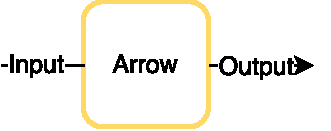
\includegraphics{images/arrow}
	\caption{Schematic depiction of an arrow.}
\end{figure}
Arrows were introduced by \citet{HughesArrows} as a general interface for computation. An arrow |arr a b| represents  a computation that converts an input |a| to an output |b|. This is defined in the |Arrow| shown in Fig.~\ref{fig:ArrowDefinition}.

\begin{figure}[t]
\centering
\parbox[c][17em]{0.49\linewidth}{%
\begin{center}
\vfill
\begin{code}
class Arrow arr where
  arr :: (a -> b) -> arr a b
  (>>>) :: arr a b -> arr b c -> arr a c
  first :: arr a b -> arr (a,c) (b,c)
\end{code}
\vfill
\end{center}
\caption{|Arrow| class definition.}
\label{fig:ArrowDefinition}
}
\parbox[c][17em]{0.49\linewidth}{%
\vfill
\centering
	{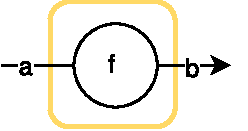
\includegraphics[scale=0.6]{images/arr}}
	{\includegraphics[scale=0.6]{images/compose}}
	{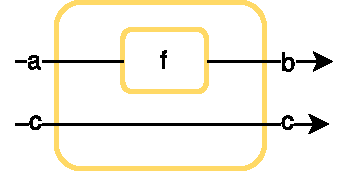
\includegraphics[scale=0.6]{images/first}}
\vfill
\caption{schematic depiction of |Arrow| combinators |arr|, |>>>| and |first|.}
}
\end{figure}
Its |arr| operation is used to lift an ordinary function to the specified arrow type, similarly to the monadic |return|. The |>>>| operator is analogous to the monadic composition  |>>=| and combines two arrows |arr a b| and |arr b c| by "wiring" the outputs of the first to the inputs to the second to get a new arrow |arr a c|. Lastly, the |first| operator  takes the input arrow from |b| to |c| and converts it into an arrow on pairs with the second argument untouched. It allows us to to save input across arrows.
\\\\
The most prominent instances of this interface are regular functions |(->)|: %(Fig.~\ref{fig:arrowfn}),
%\begin{figure}[h]
\begin{code}
instance Arrow (->) where
	arr f = f
	f >>> g = g . f
	first f = \(a, c) -> (f a, c) 
\end{code}
% \caption{Arrow instance for regular functions}
% \label{fig:arrowfn}
% \end{figure}
%%% on the verge of acceptable code
and the Kleisli type: %(Fig.~\ref{fig:arrowkleisli}).
% \begin{figure}[h]
\begin{code}
data Kleisli m a b = Kleisli { run :: a -> m b }

instance Monad m => Arrow (Kleisli m) where
	arr f = Kleisli (return . f)
	f >>> g = Kleisli (\a -> f a >>= g)
	first f = Kleisli (\(a,c) -> f a >>= \b -> return (b,c))
\end{code}%$
% \caption{Definition of the Kleisli type and the corresponding arrow instance}
% \label{fig:arrowkleisli}
% \end{figure}
\begin{figure}[h]
	\centering
	\begin{tabular}{cc}
		% \subcaptionbox
{\label{t1}}{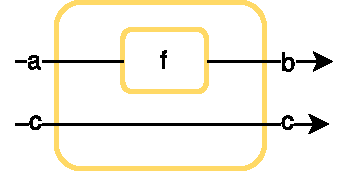
\includegraphics[width = 1.5in]{images/first}} &
		% \subcaptionbox
{\label{fig:secondImg}}{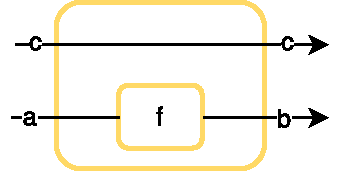
\includegraphics[width = 1.5in]{images/second}} \\
|first| & |second| \\
\midrule
		% \subcaptionbox
{}{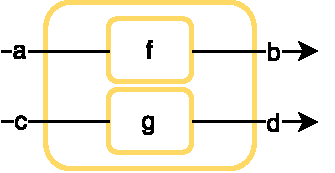
\includegraphics[width = 1.5in]{images/starstarstar}} &
		% \subcaptionbox
{}{\includegraphics[width = 1.5in]{images/andandand}}\\
|(***)|\label{fig:***Img} & |(&&&)| \label{fig:&&&Img} \\
	\end{tabular}
	\caption{Visual depiction of syntactic sugar for arrows.}
	\label{fig:syntacticSugarArrows}
\end{figure}
With this typeclass in place, Hughes also defined some syntactic sugar (Fig.~\ref{fig:syntacticSugarArrows}): The combinators |second|, |***| and |&&&|. 
The definition of |second|, the mirrored version of |first|, is:
% \begin{figure}[h]
\begin{code}
second :: Arrow arr => arr a b -> arr (c, a) (c, b)
second f = arr swap >>> first f >>> arr swap
	where swap (x, y) = (y, x)
\end{code}
% \caption{The second combinator}
% \label{fig:second}
% \end{figure}
The |***| combinator that combines |first| and |second| to handle two inputs in one arrow, is defined as
% \begin{figure}[h]
\begin{code}
(***) :: Arrow arr => arr a b -> arr c d -> arr (a, c) (b, d)
f *** g = first f >>> second g
\end{code}
% \caption{The (***) combinator}
% \label{fig:***}
% \end{figure}
, while the |&&&| combinator, that constructs an arrow which outputs two different values like |***|, but takes only one input, is:
% \begin{figure}[h]
\begin{code}
(&&&) :: Arrow arr => arr a b -> arr a c -> a a (b, c)
f &&& g = arr (\a -> (a, a)) >>> (f *** g)
\end{code}
% \caption{The (\&\&\&) combinator}
% \label{fig:&&&}
% \end{figure}
A first short example given by Hughes on how to use arrows is addition with arrows:
%|add| over arrows, which can be seen in Fig.~\ref{fig:addArrows}.
% \begin{figure}[h]
\begin{code}
add :: Arrow arr => arr a Int -> arr a Int -> arr a Int
add f g = (f &&& g) >>> arr (\(u, v) -> u + v)
\end{code}
% \caption{Add over arrows}
% \label{fig:addArrows}
% \end{figure}
% The benefit of using the |Arrow| typeclass is that any type which is shown to be an arrow can be used in conjunction with this newly created |add| combinator. Even though this example is quite simple, the power of the arrow interface immediately is clear: If a type is an arrow, it can automatically used together with every library that works on arrows. Compared to simple monads, this enables us to write code that is more extensible, without touching the internals of the specific arrows.
% \\\\
% \textit{Note: In the definitions Hughes gave in his paper, the notation |a b c| for an arrow from |b| to |c| is used. We use the equivalent definition |arr a b| for an arrow from |a| to |b| instead, to make it easier to find the arrow type in type signatures.}
%

The more restrictive interface of arrows (a monad can be \emph{anything}, an arrow is a process of doing something, a \emph{computation}) allows for more elaborate composition and transformation combinators. One of the major problems in parallel computing is composition of parallel processes.


%%% Local Variables:
%%% mode: latex
%%% TeX-master: "main"
%%% End:
